%!TEX root = main.tex
\section{Sistema de Gestión de Energía}\label{sec:sistemaGestion}

\subsection{Sistema de Almacenamiento} \label{sec:sistemaAlmacenamiento}
El sistema considerado utiliza un convertidor bidireccional AC/DC para inyectar o extraer energía de un banco de baterías y un convertidor DC/AC para extraer la energía generada por el sistema fotovoltaico. El sistema se encuentra conectado al suministro de distribución de energía, al cual se encuentran conectadas las cargas AC. En la Fig. \ref{fig:sistemaAlmacenamiento} se muestra un diagrama esquemático del sistema.
\begin{figure}
	\centering
	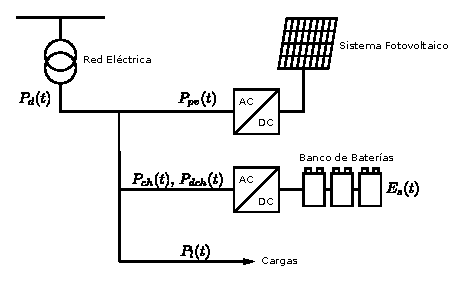
\includegraphics[width=12cm]{img/sistema_almacenamiento.eps}
	\caption{Esquema general del sistema de almacenamiento}
	\label{fig:sistemaAlmacenamiento}
\end{figure}

\subsection{Modelo Matemático del Sistema de Almacenamiento}\label{sec:modeloSistema}
En el sistema considerado las variables de interés corresponden a las potencias entregadas o consumidas por los diferentes componentes del sistema. El objetivo del problema es minimizar el costo de la energía consumida del sistema de distribución, dado que se dispone de un sistema de generación fotovoltaica y de un sistema de almacenamiento. Las variables del problema son:
\begin{align*}
	P_d(t): \quad & \text{Potencia entregada por el sistema de distribución.}\\
	P_{pv}(t): \quad & \text{Potencia entregada por el sistema fotovoltaico.}\\
	P_{ch}(t): \quad & \text{Potencia de carga del sistema de baterías.}\\
	P_{dch}(t): \quad & \text{Potencia de descarga del sistema de baterías.}\\
	P_l(t): \quad & \text{Potencia consumida por las cargas.}\\
	E_s(t): \quad & \text{Energía almacenada en las baterías.}\\
	q(t): \quad & \text{Varible binaria que representa el estado del convertidor bidireccional}\\
	& \text{(1: cargando baterías, 0: descargando baterías).}
\end{align*}

Se definen también los siguientes parámetros:
\begin{align*}
	C_d(t): \quad & \text{Precio de la energía entregada por el sistema de distribución.}\\
	\eta_{ch}: \quad & \text{Eficiencia del sistema de carga de baterías.}\\
	\eta_{dch}: \quad & \text{Eficiencia del sistema de descarga de baterías.}\\
	E_{min}, E_{max}: \quad & \text{Mínima y máxima energía almacenada en las baterías.}\\
	P_{ch}^{max}, P_{dch}^{max}: \quad & \text{Potencia máxima de carga y descarga de las baterías.}
\end{align*}

Se propone el siguiente modelo de programación matemática:
\begin{subequations}
\begin{align}
	\min_{P_d,P_{ch},P_{dch},E_s,q} \quad & \sum_{t=1}^{24} C_d(t) P_d(t)\label{eq:mod1_obj}\\
	\textrm{s.t.} \quad & E_s(t) = E_s(t-1) + \eta_{ch} P_{ch}(t-1) - \eta_{dch} P_{dch}(t-1)\label{eq:mod1_c1}\\
	& P_d(t) + P_{pv}(t) + P_{dch}(t) - P_{ch}(t) = P_l(t)\label{eq:mod1_c2}\\
	& E_s(0) = E_s(24)\label{eq:mod1_c3}\\
	& E_{min} \leq E_s(t) \leq E_{max}\label{eq:mod1_c4}\\
	& 0 \leq P_{ch}(t) \leq q(t) P_{ch}^{max}\label{eq:mod1_c5}\\
	& 0 \leq P_{dch}(t) \leq (1-q(t)) P_{dch}^{max}\label{eq:mod1_c6}\\
	& P_d(t) \leq P_l(t)\label{eq:mod1_c7}
\end{align}\label{eq:mod1}
\end{subequations}

La función objetivo mostrada en la Ec. \eqref{eq:mod1_obj} corresponde al costo de la energía entregada por el sistema de distribución. La restricción \eqref{eq:mod1_c1} relaciona el almacenamiento de energía en la batería con las potencias de carga y descarga y sus correspondientes eficiencias, asumiendo que la energía se define en unidades de kWh y que los periodos considerados corresponden a 1 hora. La restricción \eqref{eq:mod1_c2} representa el balance de energía del sistema. La restricción \eqref{eq:mod1_c3} se define para garantizar la continuidad en la operación para días sucesivos. La restricción \eqref{eq:mod1_c4} representa la capacidad mínima y máxima de carga de la batería. Las restricciones \eqref{eq:mod1_c5} y \eqref{eq:mod1_c6} definen las potencias mínima y máxima de carga y descarga de las baterías. Note que la variable binaria $q$ se utiliza aquí para garantizar que el sistema no se encuentre simultáneamente cargando y descargando las baterías. La restricción \eqref{eq:mod1_c7} define el perfil de carga como límite superior para la potencia del sistema de distribución, lo cual permite obtener un consumo balanceado a lo largo del día.

Nótese que en este modelo se asume que se conoce de antemano la potencia generada por el sistema fotovoltaico $P_{pv}$, lo cual en la práctica requiere de algoritmos de predicción para estimar los niveles de radiación sobre los paneles solares, y del conocimiento de la eficiencia de los paneles y el convertidor. En el presente trabajo se asume que $P_{pv}$ se encuentra disponible para ser utilizado en la solución del problema de optimización. También se requiere conocer el perfil de potencia del consumo de las cargas $P_l$. Dependiendo del tipo de instalación (residencial, comercial, industrial) es posible que este perfil de potencia ya se encuentre predeterminado o que dependa de las necesidades de consumo del cliente durante el día. En el presente trabajo se asume que $P_l$ se encuentra predeterminado.

La definición del costo de la energía $C_d$ puede realizarse de diferentes maneras. En el presente trabajo se utiliza la definición establecida para los cargos horarios en la resolución CREG 015 de 2018, donde se definen tres periodos de carga de la siguiente manera:
\begin{enumerate}
	\item Periodo de carga máxima (x): horas en las cuales el porcentaje de carga es mayor al 95\% de la potencia máxima.
	\item Periodo de carga media (z): horas en las cuales el porcentaje de carga es mayor al 75\% y menor o igual al 95\% de la potencia máxima.
	\item Periodo de carga mínima (y): las demás horas del día no consideradas en los periodos de carga máxima y media.
\end{enumerate}
El cálculo de los cargos horarios se obtiene resolviendo el siguiente sistema de ecuaciones:
\begin{subequations}
\begin{align}
	\frac{1}{f_{ch}} H_x P_x C_x + H_z P_z C_z &+ f_{ch} H_y P_y C_y = C_{or} \sum_{t=1}^{24} P_{or}(t)\\
	\frac{C_x}{f_{ch} C_z} &= \frac{P_x}{P_z}\\	
	\frac{C_x}{f_{ch}^2 C_z} &= \frac{P_x}{P_y}
\end{align}\label{eq:price_creg}
\end{subequations}
donde
\begin{align*}
	f_{ch}: \quad & \text{Factor para ampliar la diferencia entre los cargos horarios.}\\
	H_x, H_z, H_y: \quad & \text{Número de horas asociadas con cada uno de los periodos de carga.}\\
	P_x, P_z, P_y: \quad & \text{Potencia resultante de promediar las potencias $P_{or}$ asociadas con las}\\
	& \text{horas asignadas a cada uno de los periodos de carga.}\\
	C_x: \quad & \text{Cargo por uso para la franja de horas de carga máxima.}\\
	C_z: \quad & \text{Cargo por uso para la franja de horas de carga media.}\\
	C_y: \quad & \text{Cargo por uso para la franja de horas de carga mínima.}\\
	C_{or}: \quad & \text{Cargo por uso del operador de red.}\\
	P_{or}: \quad & \text{Perfil típico de consumo, definido por el operador de red.}
\end{align*}

Para resolver el sistema \eqref{eq:price_creg} se requiere conocer el perfil típico de consumo $P_{or}$, el cual es definido por el operador de red (OR). Una vez solucionado dicho sistema, se define el precio $C_d$ a partir de los costos de la energía y de las horas asociadas a cada uno de los niveles.

\subsection{Modelo Matemático del Sistema de Almacenamiento y Respuesta a la Demanda}\label{sec:modeloDR}
A continuación se describe una modificación al modelo \eqref{eq:mod1} para incluir un mecanismo de respuesta a la demanda (DR), el cual consiste en el recorte de consumos realizados durante las horas correspondientes a la franja de carga máxima, donde los precios de la energía son elevados, y su desplazamiento hacia las franjas de carga media y mínima, donde los precios de la energía son menores. La inclusión de este mecanismo permite disminuir los costos de la energía y realizar una redistribución de los consumos desde las horas pico hacia las horas valle, lo cual permite mejorar las condiciones operativas de la red de distribución. El método de DR implementado en este trabajo está basado en los resultados presentados en \cite{7741905}. Allí se presenta el concepto de Virtual Power Player (VPP), el cual corresponde a un agregador que agrupa múltiples generadores y consumidores, apoyando el proceso de toma de decisiones y gestionando los recursos disponibles para mejorar la operación del sistema y disminuyendo los costos para los usuarios finales.

Se definen las siguientes variables adicionales respecto a las previamente establecidas para el problema \eqref{eq:mod1}:
\begin{align*}
	P_{lp}(t): \quad & \text{Perfil de potencia de las cargas.}\\
	P_{cut_i}(t): \quad & \text{Recorte de potencia de DR en el i-ésimo nivel.}\\
	P_{sh}(t): \quad & \text{Potencia desplazada de DR.}
\end{align*}

Se definen también parámetros adicionales:
\begin{align*}
	C_{cut_i}: \quad & \text{Costo del programa DR para el i-ésimo nivel.}\\
	P_{cut_i}^{max}: \quad & \text{Máxima potencia recortada en el i-ésimo nivel.}\\
	P_{sh}^{max}: \quad & \text{Máxima potencia desplazada.}
\end{align*}

El modelo propuesto es el siguiente:
\begin{subequations}
\begin{align}
	\min_{P_d,P_{cut_i},E_b,P_{ch},P_{dch},P_{cut_i},P_{sh}} \quad & \sum_{t=1}^{24} \left(C_d(t) P_d(t) + \sum_{i \in \Omega} C_{cut_i} P_{cut_i}(t)	\right)\label{eq:mod2_obj}\\
	\textrm{s.t.} \quad & E_s(t) = E_s(t-1) + \eta_{ch} P_{ch}(t-1) - \eta_{dch} P_{dch}(t-1)\label{eq:mod2_c1}\\
	& P_d(t) + P_{pv}(t) + P_{dch}(t) - P_{ch}(t) = P_l(t) + P_{sh}(t) - \sum_{i \in \Omega} P_{cut_i}(t)\label{eq:mod2_c2}\\
	& \sum_{t=1}^{24} \sum_{i \in \Omega} P_{cut_i}(t) = \sum_{t=1}^{24} P_{sh}(t)\label{eq:mod2_c3}\\
	& E_s(0) = E_s(24)\label{eq:mod2_c4}\\
	& E_{min} \leq E_s(t) \leq E_{max}\label{eq:mod2_c5}\\
	& 0 \leq P_{ch}(t) \leq q(t) P_{ch}^{max}\label{eq:mod2_c6}\\
	& 0 \leq P_{dch}(t) \leq (1-q(t)) P_{dch}^{max}\label{eq:mod2_c7}\\
	& 0 \leq P_{cut_i}(t) \leq P_{cut_i}^{max}\label{eq:mod2_c8}\\
	& 0 \leq P_{sh}(t) \leq P_{sh}^{max}\label{eq:mod2_c9}\\
	& P_d(t) \leq P_l(t) + P_{sh}(t) - \sum_{i \in \Omega} P_{cut_i}(t)\label{eq:mod2_c10}
\end{align}\label{eq:mod2}
\end{subequations}

Para el modelo presentado en las Ecs. \eqref{eq:mod2} se ha incluido en la función objetivo \eqref{eq:mod2_obj} el costo del programa de DR, el cual permite disminuir el costo total mediante el desplazamiento de la demanda desde los periodos pico, donde el costo de la energía es elevado, hacia otros periodos horarios donde los precios son menores. La restricción \eqref{eq:mod2_c2} define la potencia consumida por las cargas en términos del perfil predeterminado de consumo $P_l$, la potencia recortada por el programa de DR en cada nivel $P_{cut_i}$, y la potencia desplazada $P_{sh}$. La restricción \eqref{eq:mod2_c3} garantiza el balance entre la potencia total recortada y la potencia desplazada. Las restricciones \eqref{eq:mod2_c8} y \eqref{eq:mod2_c9} definen los niveles máximos para la potencia recortada y desplazada. Las demás restricciones son las mismas que han sido definidas para el modelo \eqref{eq:mod1}. La restricción \eqref{eq:mod2_c10} define la potencia de las cargas ajustadas por el mecanismo de DR como límite superior para la potencia entregada por el sistema de distribución.

\section{Implementación de los Modelos y Solución}\label{sec:implementacion}
Los modelos \eqref{eq:mod1} y \eqref{eq:mod2} descritos en la sección anterior han sido formulados usando el lenguaje de programación Python y se ha utilizado el solver Gurobi \cite{gurobi} para solucionarlos. La comunicación entre el script de Python y el solver Gurobi se realiza a través de la interfaz \texttt{gurobipy}. Para realizar estos desarrollos se ha dispuesto de una licencia académica disponible de forma gratuita en su sitio web.

\subsection{Modelo 1: Sistema de Almacenamiento sin Respuesta a la Demanda}\label{sec:mod1}
En la presente sección se describe de manera general la implementación del modelo propuesto en las Ecs. \eqref{eq:mod1}, correspondiente al caso del sistema de almacenamiento con generación fotovoltaica, pero sin implementar un esquema de respuesta a la demanda. A continuación se describen las secciones de código más relevantes.

En primer lugar se importa el módulo \texttt{gurobipy}, se crea un nuevo modelo y se definen los parámetros:
\begin{minted}{python}
from gurobipy import *

# Crea un nuevo modelo
m = Model('microgrid')

# Definición de Parámetros
eta_ch  = 0.95      # Eficiencia de carga de baterías
eta_dch = 0.95      # Eficiencia de descarga de baterías
Pch_max  = 20       # Potencia máxima de carga de baterías 
Pdch_max = 20       # Potencia máxima de descarga de baterías 
Pd_max   = 50       # Potencia máxima del sistema de distribución
E_nom = 20          # Energía almacenada nominal de una batería
E_min = 0.2*Emin*5  # Energía almacenada mínima de las baterías
E_min = 0.8*Emin*5  # Energía almacenada mínima de las baterías
\end{minted}

Luego, se definen las variables del modelo:
\begin{minted}{python}
# Potencia del sistema de distribución durante cada hora [1,24]
Pd   = m.addVars(range(24), lb=0, ub=Pd_max,   name='Pd')
# Potencia de carga de las baterías durante cada hora [1,24]
Pch  = m.addVars(range(24), lb=0, ub=Pch_max,  name='Pch')
# Potencia de descarga de las baterías durante cada hora [1,24]
Pdch = m.addVars(range(24), lb=0, ub=Pdch_max, name='Pdch')
# Energía almacenada en la batería en los instantes [0,24]
Es   = m.addVars(range(25), lb=E_min, ub=E_max, name='Es')
# Variable binaria - carga o descarga de baterías
q    = m.addVars(range(24), vtype=GRB.BINARY,   name="q")
\end{minted}

Posteriormente, se definen las restricciones del problema:
\begin{minted}{python}
# Restricción (1b)
m.addConstrs((Es[t] == Es[t-1] + eta_ch*Pch[t-1] - eta_dch*Pdch[t-1] \
              for t in range(1,25)), name="C(1b)")
# Restricción (1c)
m.addConstrs((Pd[t] + Ppv[t] + Pdch[t] - Pch[t] == Pl[t] \
              for t in range(24)), name="C(1c)")
# Restricción (1d)
m.addConstr(Es[0] == Es[24], name="C(1d)")
# Restricción (1f)
m.addConstrs((Pch[t] <= q[t]*Pch_max for t in range(24)), name="C(1f)")
# Restricción (1g)
m.addConstrs((Pdch[t] <= (1-q[t])*Pdch_max for t in range(24)), name="C(1g)")	
\end{minted}

Finalmente, se define la función objetivo, se ejecuta la optimización y se recuperan las soluciones:
\begin{minted}{python}
# Función objetivo (1a) 
m.setObjective(quicksum(Cd[t]*Pd[t] for t in range(24)), GRB.MINIMIZE)
# Actualiza el modelo con los cambios
m.update()
# Ejecuta el optimizador
m.optimize()
# Recupera las soluciones
if m.status == GRB.Status.OPTIMAL:
    Pd_sol   = m.getAttr('x', Pd)
    Pch_sol  = m.getAttr('x', Pch)
    Pdch_sol = m.getAttr('x', Pdch)
    Es_sol   = m.getAttr('x', Es)	
\end{minted}

\subsection{Modelo 2: Sistema de Almacenamiento con Respuesta a la Demanda}\label{sec:mod2}
Ahora se procede a describir de manera general la implementación del modelo \eqref{eq:mod2}, correspondiente al caso del sistema de almacenamiento con generación fotovoltaica y con un esquema de respuesta a la demanda.
Se importa el módulo \texttt{gurobipy}, se crea el nuevo modelo y se definen los parámetros. Note que se aquí se configuran los niveles máximos de potencia a recortar en cada nivel del programa de DR, y los costos asociados a cada uno.
\begin{minted}{python}
# Crea un nuevo modelo
m = Model('microgrid')

# Definición de Parámetros
eta_ch  = 0.95      # Eficiencia de carga de baterías
eta_dch = 0.95      # Eficiencia de descarga de baterías
Pch_max  = 20       # Potencia máxima de carga de baterías 
Pdch_max = 20       # Potencia máxima de descarga de baterías 
Pd_max   = 50       # Potencia máxima del sistema de distribución
E_nom = 20          # Energía almacenada nominal de una batería
E_min = 0.2*Emin*5  # Energía almacenada mínima de las baterías
E_min = 0.8*Emin*5  # Energía almacenada mínima de las baterías
Pcut_max = 20       # Potencia máxima recortada de DR nivel 1
Psh_max = 100       # Potencia máxima desplazada por DR
Ccut = [38, 56, 114] # Precio del programa DR para cada nivel
\end{minted}

Ahora, se definen las variables del problema:
\begin{minted}{python}
# Potencia del sistema de distribución durante cada hora [1,24]
Pd   = m.addVars(range(24), lb=0, ub=Pd_max,   name='Pd')
# Potencia de carga de las baterías durante cada hora [1,24]
Pch  = m.addVars(range(24), lb=0, ub=Pch_max,  name='Pch')
# Potencia de descarga de las baterías durante cada hora [1,24]
Pdch = m.addVars(range(24), lb=0, ub=Pdch_max, name='Pdch')
# Energía almacenada en la batería en los instantes [0,24]
Es   = m.addVars(range(25), lb=E_min, ub=E_max, name='Es')
# Recorte de potencia de DR en el i-ésimo nivel
Pcut = m.addVars(len(Ccut),range(24), lb=0, ub=Pcut_max, name='Pcut')
# Potencia desplazada del programa de DR
Psh  = m.addVars(range(24), lb=0, ub=Psh_max,   name='Psh')
# Variable binaria - carga o descarga de baterías
q    = m.addVars(range(24), vtype=GRB.BINARY, name="q")
\end{minted}

Posteriormente, se definen las restricciones del problema:
\begin{minted}{python}
# Restricción (3b)
m.addConstrs((Es[t] == Es[t-1] + eta_ch*Pch[t-1] - eta_dch*Pdch[t-1]\
    for t in range(1,25)), name="C(3b)")
# Restricción (3c)
m.addConstrs((Pd[t] + Ppv[t] + Pdch[t] - Pch[t] == Pl[t] + Psh[t]\
  - quicksum(Pdr[i,t] for i in range(len(Ccut))) for t in range(24)), name="C(3c)")
# Restricción (3d)
m.addConstr(quicksum(Pcut1[t] + Pcut2[t] + Pcut3[t] for t in range(24))\
    == quicksum(Psh[t] for t in range(24)), name="C(3d)")
# Restricción (3e)
m.addConstr(Es[0] == Es[24], name="C(3e)")
# Restricción (3g)
m.addConstrs((Pch[t] <= q[t]*Pch_max for t in range(24)), name="C(3g)")
# Restricción (3h)
m.addConstrs((Pdch[t] <= (1-q[t])*Pdch_max for t in range(24)), name="C(3h)")
\end{minted}

Finalmente, se define la función objetivo, se actualiza el modelo con los cambios realizados y se ejecuta el optimizador. Luego se recuperan las soluciones.
\begin{minted}{python}
# Función objetivo (3a)
m.setObjective(quicksum(Cd[t]*Pd[t] + quicksum(Ccut[i]*Pdr[i,t]\
    for i in range(len(Ccut))) for t in range(24)), GRB.MINIMIZE)
# Actualiza el modelo con los cambios
m.update()
# Ejecuta el optimizador
m.optimize()
# Recupera las soluciones
if m.status == GRB.Status.OPTIMAL:
    Pd_sol = m.getAttr('x',Pd)
    Pch_sol = m.getAttr('x',Pch)
    Pdch_sol = m.getAttr('x',Pdch)
    Es_sol = m.getAttr('x',Es)
    Psh_sol = m.getAttr('x',Psh)
    Pcut_sol = m.getAttr('x',Pcut)
\end{minted}

\subsection{Cálculo de los Precios de la Energía}\label{sec:creg}
Como se describió en la sección anterior, los precios de la energía se calculan con base en lo especificado en la resolución CREG 015/2018, capítulo 9. Allí se describe un conjunto de periodos, los cuales se definen con base en un perfil de carga típico establecido por el operador de red para diferentes niveles de tensión. Para solucionar el problema se ha utilizado el módulo  A continuación se muestra la implementación del sistema presentado en las Ecs. \eqref{eq:price_creg}:

\begin{minted}{python}
import numpy as np

# Definición del perfil de carga típico
loadProfile = [60,65,70,70,75,80,80,80,80,80,75,75,75,80,85,90,90,95,\
               100,100,95,85,80,65]
Pi  = 0.01*np.array(loadProfile)
Cor = 550   # Cargo por uso del operador de red
fch = 2     # Factor para ampliar la diferencia entre cargos horarios

# Establece las horas asociadas a cada periodo de carga
indx = np.where((Pi>=0.95))[0]
indz = np.where((Pi<0.95) & (Pi>=0.75))[0]
indy = np.where((Pi<0.75))[0]

# Calcula el número de horas asociadas a cada periodo de carga
Hx = len(indx)
Hz = len(indz)
Hy = len(indy)

# Potencia promedio asociada a cada periodo de carga
Px = np.mean(Pi[indx])
Pz = np.mean(Pi[indz])
Py = np.mean(Pi[indy])

# Construye las matrices del problema
A = np.array([[Hx*Px/fch,Hz*Pz,fch*Hy*Py],[1/fch,-Px/Pz,0],[1/(fch*fch),0,-Px/Py]])
b = np.array([[Dt*np.sum(Pi)],[0],[0]])

# Calcula la solución del problema
x = np.linalg.solve(A,b)

# Recupera la solución del problema
Cd = np.zeros(24)
Cd[indx] = x[0]
Cd[indz] = x[1]
Cd[indy] = x[2]
\end{minted}

\subsection{Perfil de Potencia Exportado para la Interfaz de Medición}\label{sec:exportarDatos}
El mecanismo que se ha diseñado para comunicar el sistema de gestión con la interfaz de medición es a través de un documento de texto plano.
Una vez se ha encontrado la solución al problema de optimización presentado en la sección anterior, los datos son exportados a un archivo con caracteres de separación. A continuación se presenta el código desarrollado para exportar los datos:
\begin{minted}{python}
import pandas as pd
import datetime

data = {'H': [datetime.time(i,0).strftime("%H:%M") for i in range(24)],\
       'Pch': Pch[:-1], 'Pdch': Pdch[:-1], 'Pd': Pd[:-1]}
df = pd.DataFrame(data)
df.to_csv(fileName, sep=';', index=False, line_terminator=';\n', date_format="%H:%M")
\end{minted}

Una muestra del archivo generado se muestra a continuación:
\begin{minted}{python}
H;Pch;Pdch;Pd;
00:00;0.0;0.0;21.0859;
01:00;0.0;0.0;20.2583;
02:00;0.0;0.0;20.1845;
...
22:00;0.0;0.0;29.0459;
23:00;0.0;0.0;24.1434
\end{minted}

La información contenida en este archivo tiene cuatro columnas: la hora, la potencia de carga de las baterías, la potencia de descarga de las baterías y la potencia de la red de distribución. Esta información es usada para configurar los set-points del sistema desde la interfaz de usuario.

\section{Resultados}\label{sec:resultados}
A continuación se presentarán los resultados obtenidos al encontrar la solución para los modelos presentados en las secciones \ref{sec:mod1} y \ref{sec:mod2} respecto a un caso base, correspondiente al costo de la energía entregada por el sistema de distribución para alimentar las cargas de acuerdo con el perfil establecido y con los precios definidos en la sección \ref{sec:creg}.

\subsection{Escenario 1: Sistema de Almacenamiento sin Respuesta a la Demanda}\label{sec:escenario1}
En la Fig. \ref{fig:escenario1} se muestran los resultados para el primer escenario, el cual corresponde a la solución del problema de optimización para el modelo presentado en las Ecs. \eqref{eq:mod1}.

En la primera subfigura, se muestra un ejemplo de la curva típica de carga definido por el operador de red, expresada en porcentaje del valor máximo de carga, y el costo calculado al resolver las Ecs \eqref{eq:price_creg}. En este caso el cargo por uso del operador de red $C_{or} = 550$.

En la segunda subfigura, se presenta la potencia entregada por el sistema de distribución $P_d$, la potencia generada por el sistema fotovoltaico $P_{pv}$ y la potencia consumida por las cargas $P_l$. Note que el perfil de potencia $P_l$ presenta el patrón común de consumo en instalaciones residenciales, donde durante las horas al final del día y en la madrugada la potencia requerida es mínima, mientras que se observan valores de potencia intermedios durante la mañana y la tarde y un pico elevado de consumo cuando cae la noche.
En este caso se observa que no toda la potencia requerida por las cargas es suministrada por el sistema de distribución, sino que se aprovecha la potencia generada por el sistema fotovoltaico.

En la tercera subfigura se observa la operación del sistema de almacenamiento, donde la potencia $P_{pv}$ se usa hacia las horas de la mañana y el medio día para realizar la carga de las baterías, y posteriormente se descargan para suministrar parte de la energía requerida en las horas pico de consumo.

El costo total de la energía para el caso base, donde no se cuenta con un sistema de almacenamiento ni de generación fotovoltaica, se obtiene multiplicando el costo de la energía por el consumo requerido por las cargas. En este caso es igual a \$506084.45. Cuando se cuenta con un sistema de almacenamiento y generación fotovoltaica el costo total de la energía es igual a \$374751.91, lo cual representa una reducción del 26\%. Esta reducción en el costo total se obtiene gracias al aprovechamiento de la energía generada durante el día para ser utilizada durante las horas pico.

\begin{figure}
	\centering
	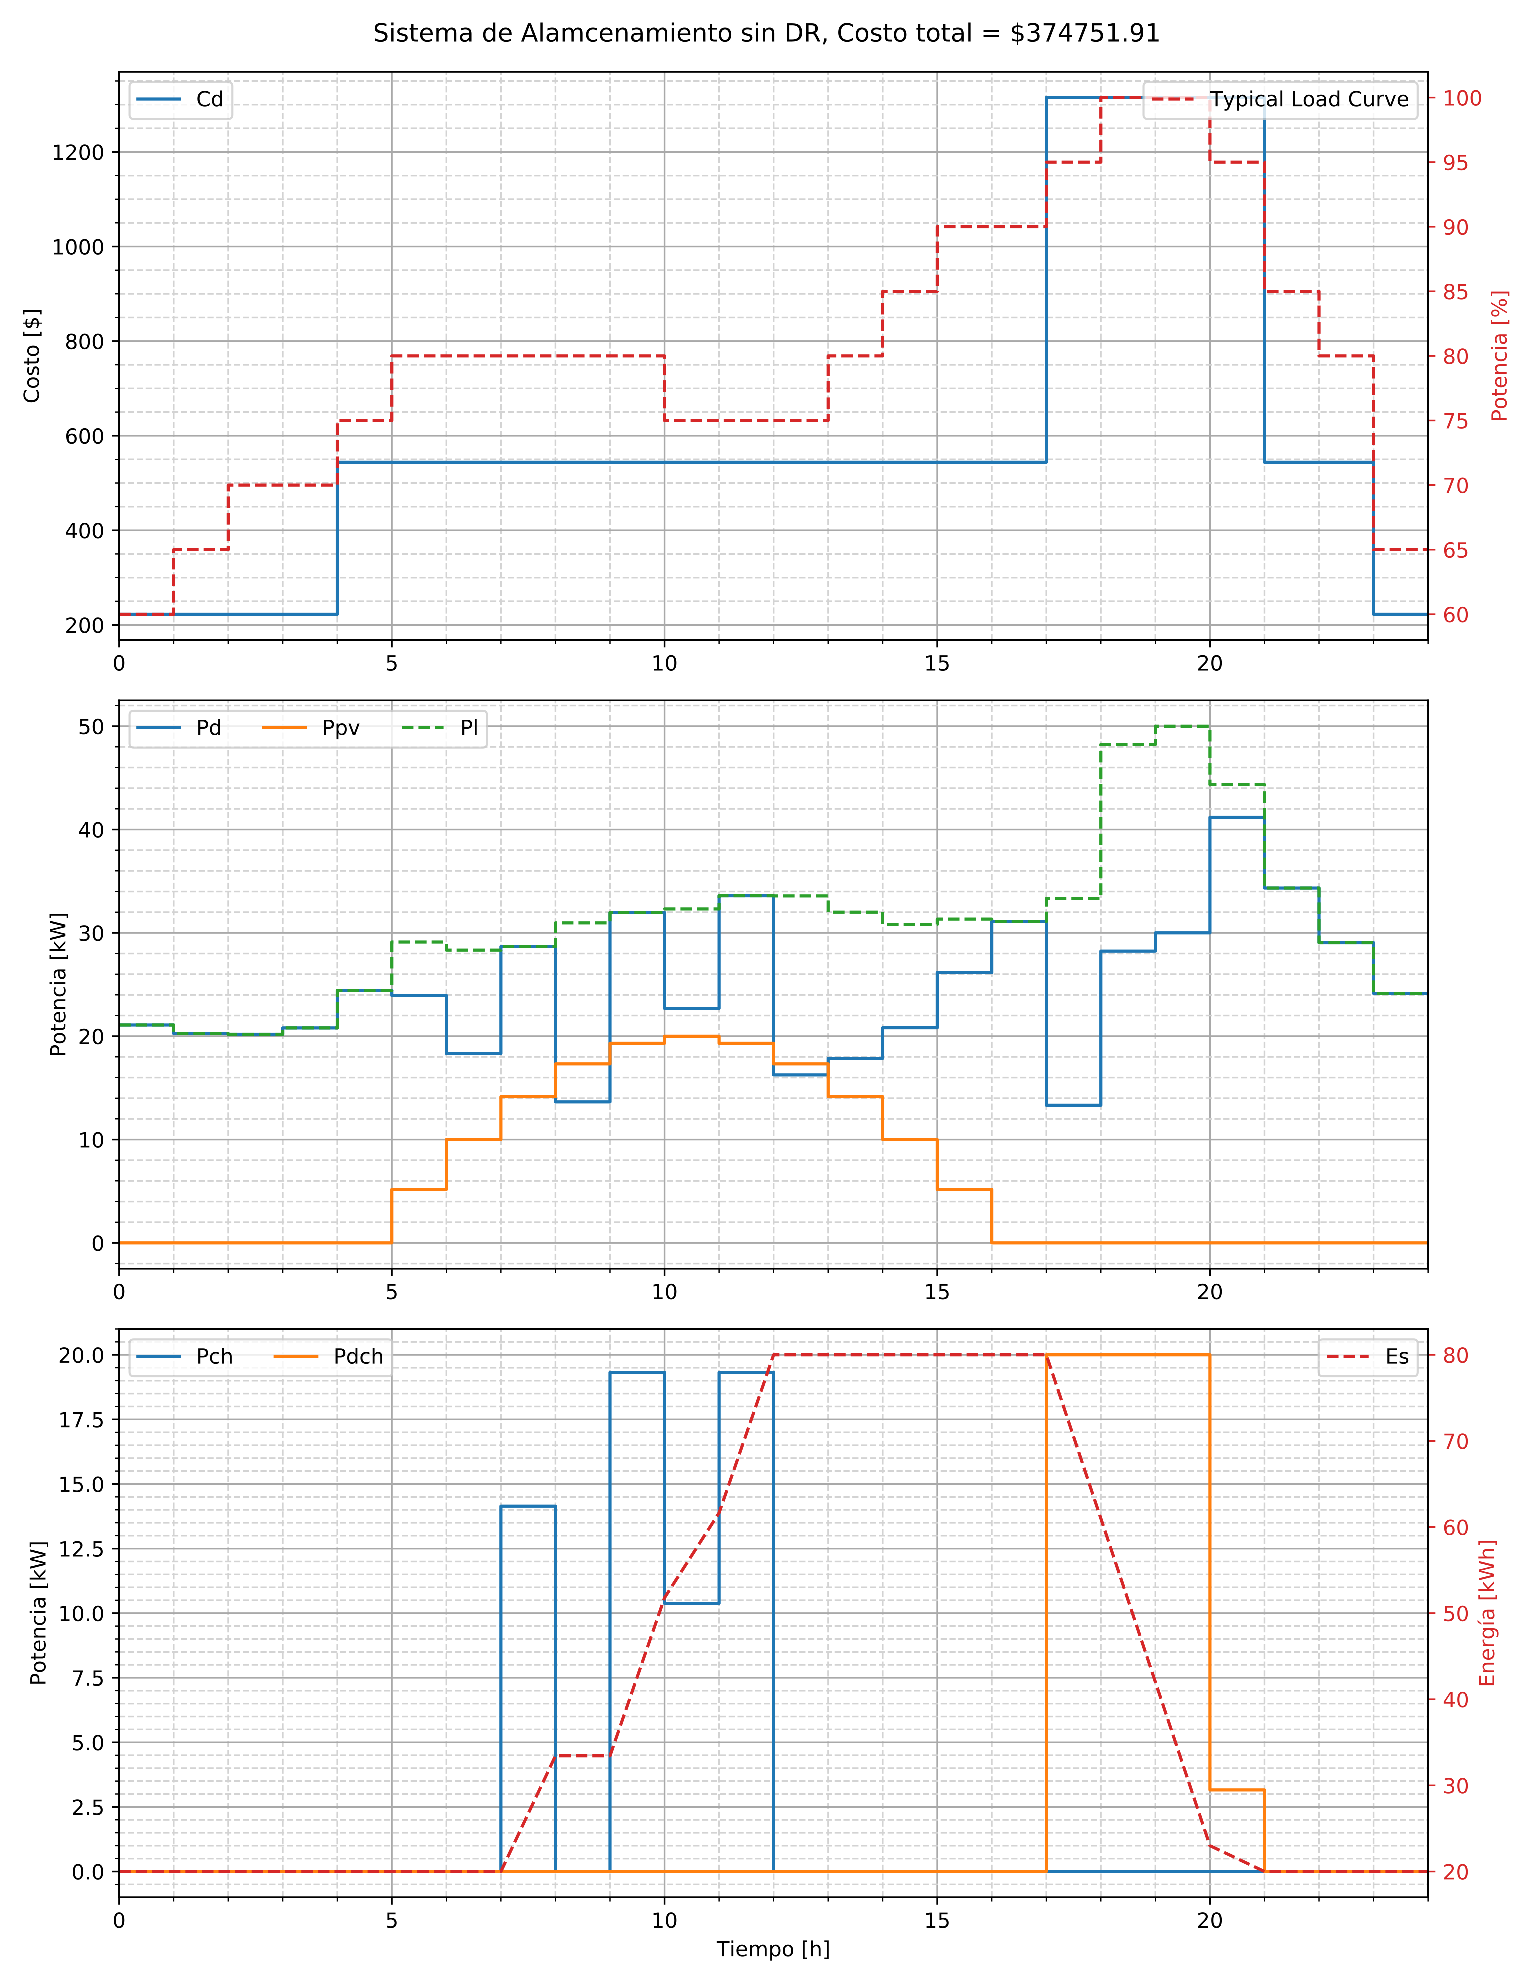
\includegraphics[width=16cm]{img/escenario1.eps}
	\caption{Escenario 1: Resultados para el sistema con generación y almacenamiento pero sin respuesta a la demanda.}
	\label{fig:escenario1}
\end{figure}

\subsection{Escenario 2: Sistema de Almacenamiento con Respuesta a la Demanda}\label{sec:escenario2}
En la Fig. \ref{fig:escenario2} se muestran los resultados para el segundo escenario, el cual corresponde a la solución del problema de optimización para el modelo presentado en las Ecs. \eqref{eq:mod2}.

En la primera subfigura, se muestran las mismas señales de carga típica y costo calculado por el operador de red empleados en el escenario 1.

En la segunda subfigura, se presenta la potencia entregada por el sistema de distribución $P_d$, la potencia generada por el sistema fotovoltaico $P_{pv}$, y el perfil de potencia requerida por las cargas $P_l$. También se presenta el nuevo perfil de potencia consumida por las cargas que se obtiene del programa de DR, donde los consumos durante las horas pico han sido recortados y desplazados hacia otras franjas horarias donde los precios de la energía son menores. En la tercera subfigura se pueden observar los recortes de energía obtenidos para los dos primeros niveles, los cuales logran disminuciones considerables en las horas pico y durante algunas horas intermedias. Dichos consumos han sido desplazados hacia las franjas de carga mínima, donde los precios de la energía son significativamente menores.

Finalmente, en la cuarta subfigura se observa la operación del sistema de almacenamiento, donde nuevamente la potencia generada por el sistema fotovoltaico se aprovecha para realizar la carga de las baterías y esta energía también será utilizada para satisfacer la porción restante de potencia requerida durante la franja de carga máxima. 

Para este escenario el costo total de la energía es igual a \$247736.74, lo cual corresponde a una disminución del 51\% respecto al costo base, y del 33\% respecto al caso presentado en el escenario 1. Estos resultados muestran que una estrategia combinando el uso del sistema de generación y almacenamiento con un mecanismo de respuesta a la demanda tiene el potencial para mejorar la eficiencia en la operación del sistema de distribución al mismo tiempo que se  disminuyen los costos para los clientes finales.

\begin{figure}
	\centering
	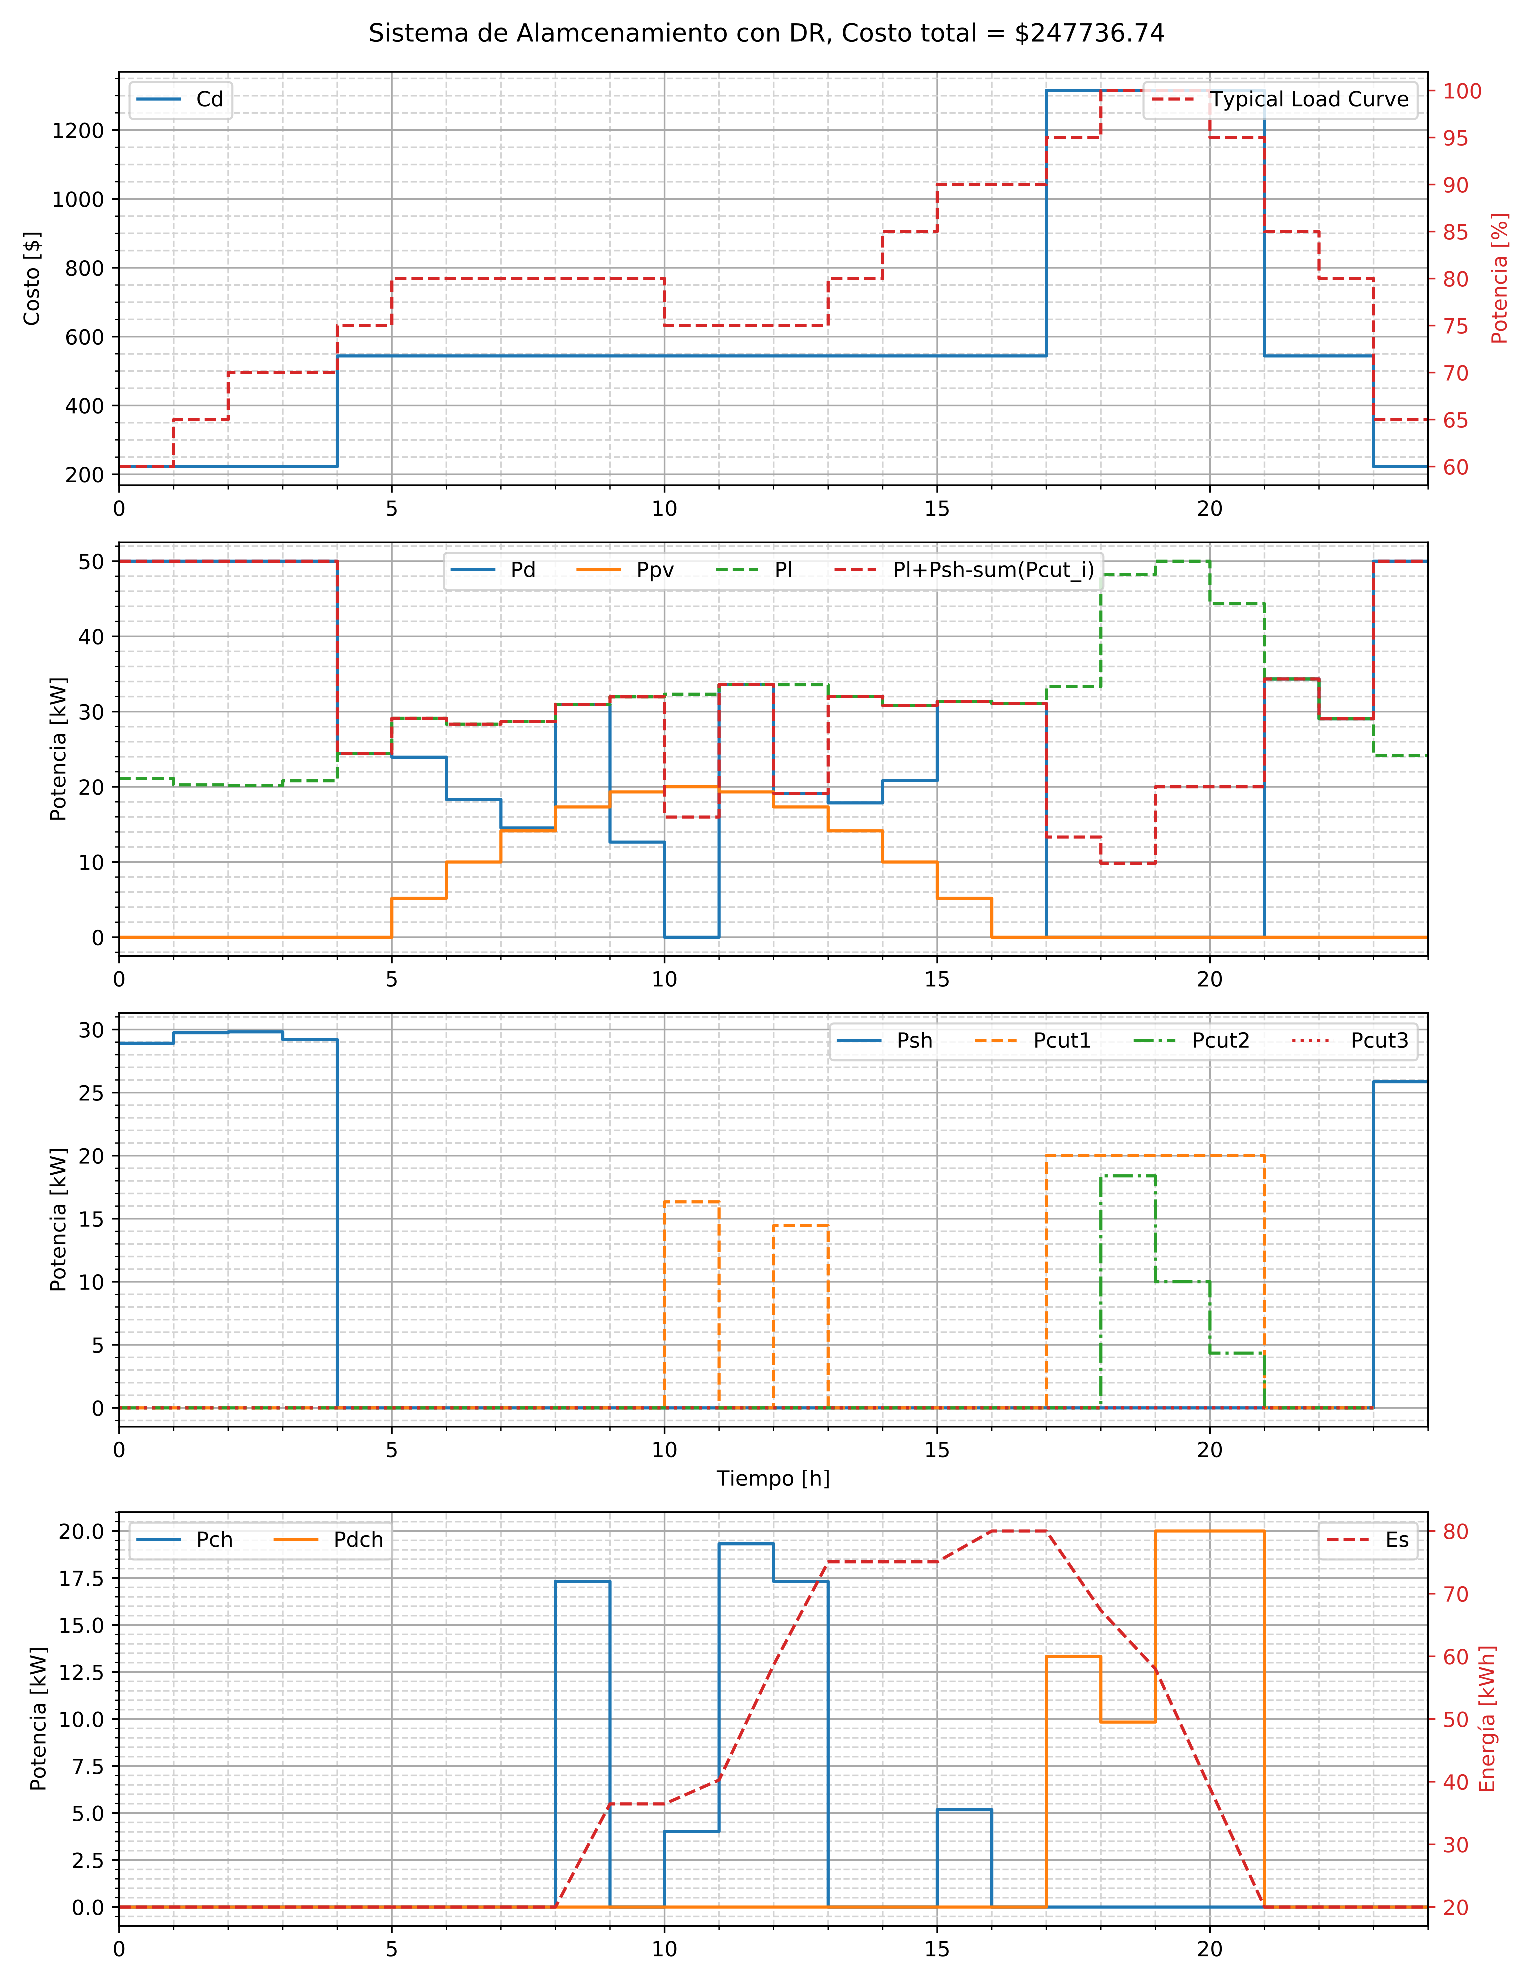
\includegraphics[width=16cm]{img/escenario2.eps}
	\caption{Escenario 2: Resultados para el sistema con generación, almacenamiento y respuesta a la demanda.}
	\label{fig:escenario2}
\end{figure}
